\documentclass[12pt,twoside,openright, fleqn]{report} 


\usepackage{preamble}



\setlength{\marginparwidth}{0pt}
\setlength{\oddsidemargin}{20pt}
\setlength{\textwidth}{450pt}


%%%%

\newcommand{\bs}[1]{\boldsymbol{#1}}
\newcommand{\wrong}[1]{(\textcolor{red}{not #1})}
\newcommand{\note}[1]{{(\textcolor{red}{#1})}}
\newcommand\emptypage{
\newpage
\thispagestyle{empty}
\mbox{}
\newpage
}

\def\mytitle{BTP-1}
\def\myname{Himanshu Sharma}
\def\mydegree{Dual Degree (B.Tech + M.Tech)}
\def\mysupervisor{Dr. Jeevanjyoti Chakraborty}
\def\myrollno{21ME33001}
\def\mydep{Mechanical Engineering}
\def\mydegreedate{Autumn Semester, 2024-2025}
%%%%


\begin{document}
%\layout

%this baselineskip gives sufficient line spacing for an examiner to easily
%markup the thesis with comments
\baselineskip=18pt plus1pt

%set the number of sectioning levels that get number and appear in the contents
\setcounter{secnumdepth}{3}
\setcounter{tocdepth}{3}
% \maketitle


% \pagebreak
\pagenumbering{roman}
\thispagestyle{empty}
\begin{center}
    { \large {\bfseries {\mytitle}} \par}
\vspace{3\baselineskip}
    {\textit{Thesis submitted to the} \\ \textit{Indian Institute of Technology Kharagpur} \\ \textit{In partial fulfillment for the award of the degree} \par}
\vspace{\baselineskip}
    {\textit{of} \par}
\vspace{\baselineskip}
    {\large \bf \mydegree \par} 
\vspace{\baselineskip}
    {\textit{by} \par}
\vspace{\baselineskip}
    {{\large {\bf \myname \\ \myrollno}} \par}
%\vspace{-0.1\baselineskip}
%    {{\large {\bf \myrollno}} \par}
\vspace{1.5\baselineskip}
    {Under the guidance of \par}
\vspace{\baselineskip}
    {{\large \bf \mysupervisor} \par}
\vspace{1.5\baselineskip}
    {\begin{figure}[!h] 
	\centering
	\includegraphics[width=32mm]{./iitkgplogo.JPG} 
     \end{figure}
    }
%{\large \vspace*{1ex}
%\vspace{\baselineskip}
    {\bf \MakeUppercase{\mydep} \par}
\vspace*{1ex}
    {\bf \uppercase{Indian Institute of Technology Kharagpur} \par}
%\vspace*{25mm}
%    {{\submittedtext} \par}
%\vspace*{2ex}
    {\Large \mydegreedate \par}
    {\copyright $\,$\myname. All rights reserved.}
  \end{center}



\addcontentsline{toc}{chapter}{Certificate}
\begin{center}
{\Large {\bf \uppercase{Certificate}}}
\end{center}
\thispagestyle{plain}
\noindent This is to certify that the thesis entitled {\bf \mytitle}, submitted by {\bf \myname} to the Indian Institute of Technology Kharagpur, is a record of bona fide research work under my supervision and I consider it worthy of consideration for the award of the degree of {\bf \mydegree} of the Institute. 
\vspace{3\baselineskip}
\begin{flushright}
\begin{minipage}[c]{0.4\textwidth}
\centering
\hrule 
\vspace{0.5\baselineskip}
{\Large \bf Supervisor} \\
\end{minipage}
\end{flushright}
\vspace{\baselineskip}

{\large \bf Date: }


\addcontentsline{toc}{chapter}{Declaration}
\begin{center}
{\Large {\bf \uppercase{Declaration}}}
\end{center}
\thispagestyle{plain}
\noindent I certify that 
%\vspace{1\baselineskip}

\begin{itemize}
\item[a.] The work contained in the thesis is original and has been done by myself under the general supervision of my supervisor.
\item[b.] The work has not been submitted to any other Institute for any degree or diploma. 
\item[c.] I have followed the guidelines provided by the Institute in writing the thesis. 
\item[d.] I have conformed to the norms and guidelines in the Ethical Code of Conduct of the Institute. 
\item[e.] Whenever I have used materials (data, theoretical analysis, and text) from other sources, I have given due credit to them by citing them in the text of the thesis and giving their details in the references. 
\item[f.] Whenever I have quoted written materials from other sources, I have put them under quotation marks and given due credit to the sources by citing them and giving required details in the references. 
\end{itemize}

\begin{flushright}
\begin{minipage}[c]{0.5\textwidth}
%\centering
%\hrule 
\vspace{3\baselineskip}
{\large \bf Signature of the Student} \\
\end{minipage}
\end{flushright}

\vspace{\baselineskip}

%{\large \bf Date: }


\addcontentsline{toc}{chapter}{Acknowledgements}
\thispagestyle{plain}
\begin{center}
{\Large \bf \uppercase{Acknowledgements}}
\end{center}
plenty of waffle, plenty of waffle, plenty of waffle, plenty of waffle,
plenty of waffle, plenty of waffle, plenty of waffle, plenty of waffle.



\addcontentsline{toc}{chapter}{List of Symbols and Abbreviations}
\begin{center}
{\Large \bf \uppercase{List of Symbols and Abbreviations}}
\end{center}
 

\addcontentsline{toc}{chapter}{Abstract}
\begin{center}
{\Large \bf \uppercase{Abstract}}
\end{center}
plenty of waffle, plenty of waffle, plenty of waffle, plenty of waffle,
plenty of waffle, plenty of waffle, plenty of waffle, plenty of waffle.
 

\tableofcontents            % generate and include a table of contents


\clearpage


\pagenumbering{arabic}
\documentclass[../main.tex]{subfiles}


\begin{document}
\textbf{introduction}
\end{document}
\chapter{Problem Description}
Consider a thin film of Silicon with height $H$ and length $L$. All the loadings and geometry are independent of the third direction; hence, the problem is formulated using the plane strain assumption. There is an existing solid electrolyte interphase (SEI) layer on top of the Silicon film with a height of $H_{\rm{SEI}}$. The origin is placed at the middle of the bottom face of the Silicon film, as shown in figure \ref{fig:probDesc}. The Si thin film's bottom face is considered rigidly fixed to a metallic substrate. The left and right faces are considered to have a roller-type boundary condition for both Si and SEI. A uniform flux of Li-ions from the top surface of SEI is present. 
\begin{figure}[H]
    \centering
    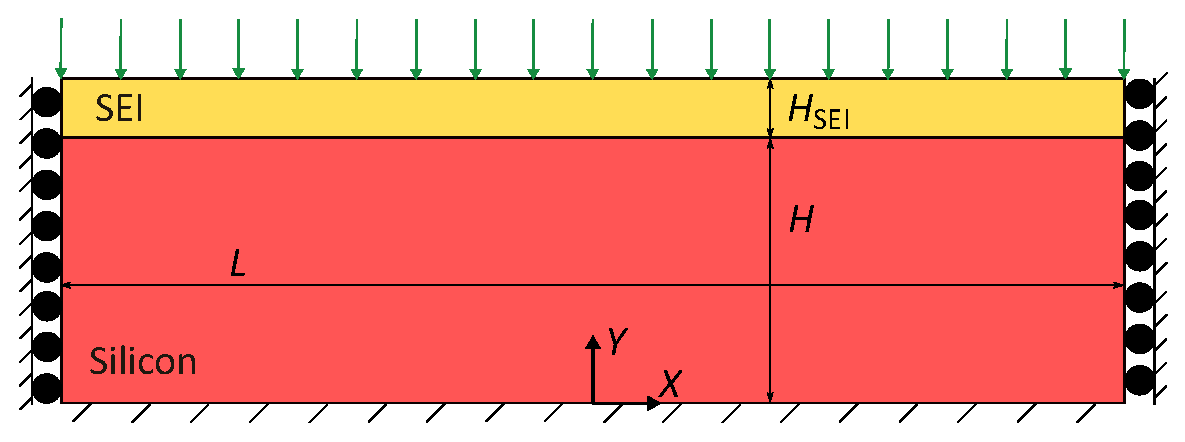
\includegraphics[width=\textwidth]{figures/probDescFigs/drawing.eps}
    \caption{Schematic of the problem showing geometric parameters and boundary conditions.}
    \label{fig:probDesc}
\end{figure}
SEI is considered completely permeable to Li-ions. So the flux directly enters the Silicon without any diffusion in the SEI. And the diffusion in Si leads to a stress field. In the literature, this is termed diffusion-induced stress (DIS). The stress field, in turn, affects the process of diffusion called stress-enhanced diffusion (SED). \\
Due to the large deformation of the Si during lithiation/delithiation, it is necessary to formulate the problem with finite deformation theory with an elastoplastic constitutive behavior. In the present study, Si is considered to exhibit a viscoplastic nature. The SEI is assumed to undergo only elastic deformation. The constitutive law for the elastic regime is isotropic and concentration-dependent for Li$_\chi$Si and constant for SEI. 
For Mechanical equilibrium, a quasi-static model is employed. This leads to a two-way coupled system of PDEs which is then solved using the finite element method in COMSOL multiphysics.

\chapter{Mathematical Formulation}

\section{Kinematics}
Consider a certain particle, initially located at the coordinate $\X$. During deformation, this particle follows a path 
\begin{gather}
\x = \x(\X,t).
\end{gather}
Let $\u(\X, t)$ be the displacement of the material particle located at $\X$. Then
\begin{gather}
    \u(\X, t) = \x(\X, t) - \X.
\end{gather}
The total deformation gradient and Green-Lagrange strain are denoted by $\F$ and $\E$, respectively. Therefore, 
\begin{align}
    \F &= \pdiff{\x}{\X} = \nablaX \u + \I, \\
    \E &= \fc{1}{2}(\F^\T \cdot \F - \I)
\end{align}
where $\I$ is the second order isotropic tensor.

Let $\{\hat{\bm{e}}_1, \hat{\bm{e}}_2, \hat{\bm{e}}_3\}$ be the orthonormal basis in the reference configuration. corresponding components of $\X$ are denoted by $X$, $Y$ and $Z$ and that of $\u$ by $u$, $v$ and $w$. In the present study, plane strain deformation is assumed. Therefore, the components of F are given by \citep{2009ContMechLai} 
\begin{align}
[\F] = 
\begin{bmatrix}
       1 + \pdiff{u}{X} && \pdiff{u}{Y} && 0 \\
       \pdiff{v}{X} && 1 + \pdiff{v}{Y} && 0 \\
       0 && 0 && 1
\end{bmatrix} = \tensor{F}. \label{eq:F_tensor}
\end{align}
Both Inelastic and elastic deformation gradients are considered to be finite \citep{2011JMPSBower}. Hence, a multiplicative decomposition of $\F$ into elastic and inelastic deformation is necessary. As shown in \ref{fig:decomposition}, the body is first considered to reach an intermediate stress free state and then it undergoes an elastic deformation to reach the current configuration. As derived by \citet{1969Lee}, the total deformation gradient   
\begin{gather}
\F = \F^{\el} \cdot  \F^{\inel} \label{eq:F_decomposition} \\
\text{where, } \F^{\el} = \pdiff{\x}{\x_I} \text{ and } \F^{\inel} = \pdiff{\x_{I}}{\X} \nonumber
\end{gather}
\begin{figure}[H]
    \centering
    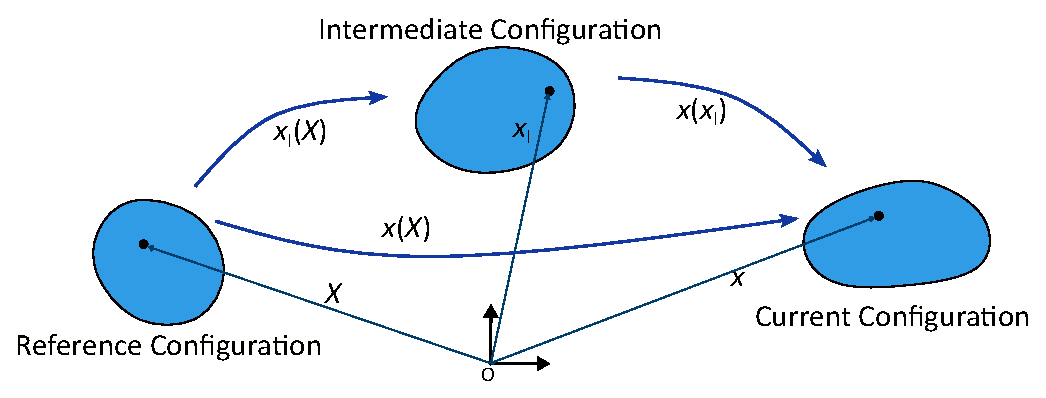
\includegraphics[width=\textwidth]{figures/decomposition.eps}
    \caption{Decomposition of deformation gradient into elastic and inelastic part.}
    \label{fig:decomposition}
\end{figure}
$\F^{\el}$ and $\F^{\inel}$ denote the deformation gradients due to elastic deformation and inelastic deformation respectively.

The inelastic deformation gradient tensor, $\F^{\inel}$, has contribution from two sources. It is further decomposed as 
\begin{gather}
    \F^\inel = \F^\c \cdot \F^\p. \label{eq:Finel_decomposition}
\end{gather}
Where $\F^\c$ and $\F^\p$ are deformation gradients due to diffusion and plastic flow, respectively.

\section{Viscoplastic Flow}
A viscoplastic constitutive relation of the following form is considered.
\begin{gather}
\DP = \pdiff{G(\sigmaeff)}{\DCS}
\end{gather}
Where $\DP$ is the rate dependent plastic deformation tensor, $G(\sigmaeff)$ is the flow potential, $\sigmaeff$ is the von Mises stress and $\DCS$ is the deviatoric part of Cauchy stress tensor. Various studies \citep{2011JMPSBower,2012JMPSCui} have adopted a power law of following for flow potential
\begin{align}
G(\sigmaeff) &= \fc{\sigmaf \dZEROdot}{\mathrm{m}+1}\left(\fc{\sigmaeff}{\sigmaf}-1\right)^{\mathrm{m}+1}\heavi. \\
\Rightarrow \mathbf{D}^{\rm{P}} &= \fc{3 \DCS \dZEROdot}{2 \sigmaeff}\left(\fc{\sigmaeff}{\sigmaf}-1\right)^{\mathrm{m}}\heavi.
\end{align}
where $\sigmaeff$ is the effective von Mises stress, defined in section \ref{section:MechEqbm}, H is the unit step function, $\sigmaf$ is the yield strength of Silicon, m is the stress exponent for plastic flow and $\dZEROdot$ is the strain rate for plastic flow. \note{read about the following equation from \citep{2005JMPSGurtin,2005IJPGurtin}}
\begin{align}
\mathbf{D}^{\rm{P}} &= \F^{\el} \F^{\rm{c}} \dot{\F}^\p \inv{\F^\p} \inv{\F^{\rm{c}}} \inv{\F^{\el}}  \\
\Rightarrow \dot{\F}^\p &= \inv{J} \fc{3}{2} \fc{\Mel \F^\p}{\sigmaeff} \dZEROdot \left( \fc{\sigmaeff}{\sigmaf} - 1 \right)^\m \heavi  \\
\text{where }\Mel &= J (\F^\el)^\T \DCS (\F^\el)^\mT \label{eq:M_tensor} \\
J &= \mathrm{det}(\F) 
\end{align}
$\Mel$ is the deviatoric part of Mandel stress \citep{1971Mandel}. The expression for Mandel stress is 
\begin{nonumbereq}
\mathbf{M}^{\el} = J (\F^{\el})^{\T} \CS \invT{F^{\el}}.
\end{nonumbereq}
Attributing to the assumption of plane strain, $\F^{\rm{p}}$ is considered to be of the following form:
\begin{gather}
    [\F^\p] = \tensor{\lambda}.
\end{gather}
Since, det($\F^\p$) = 1
\begin{gather}
     \lamzz = 1/(\lamxx \lamyy - \lamxy \lamyx).
\end{gather}



\section{Diffusion Induced Deformation}
The compound formed between Lithium and Silicon is of the form $\text{Li}_{\chi}$Si. Let the stoichiometric concentration and maximum concentration of Lithium ions per atom of Silicon be denoted by $\chi_0$ and $\chi_{\rm{max}}$. Defining a non-dimensional measure of the Li-ions concentration as $\tc  = (\chi-\chi_{0})/\xmax$. since, $\chi_{0}$ is the stoichiometric ratio it signifies the stress free state of the particle and hence, $\tc$ is a measure of the deviation of the particle from undeformed state. The deformation due to lithiation is quantified by an isotropic deformation gradient denoted by $\F^\c$ and given by
\begin{gather}
    \F^\c = (\jc)^{1/3} \I
\end{gather}
where \begin{nonumbereq}\jc = 1 + 3 \eta \xmax \tc\end{nonumbereq} is the volumetric change experienced by the Silicon film upon insertion of Li-ions. $\eta$ is a material parameter giving rate of change in volume w.r.t. $\tc$. It may be noted that as $\tc$ approaches 1, $\mathrm{det}(\F^\c)$ approaches 4. Therefore the body undergoes a volumetric change of about 300\% due to diffusion of Li-ions, justifying the use of large deformation analysis.

\section{Mechanical Equilibrium } \label{section:MechEqbm}
From equations \ref{eq:F_decomposition} and \ref{eq:Finel_decomposition},
\begin{align}
    \F^{\el} &=  \F \cdot \inv{\F^{\p} \cdot \F^{\c}}. \label{eq:Fel_tensor}
\end{align}
The elastic Green-Lagrange strain
\begin{nonumbereq}
\E^{\el} = \fc{1}{2} \left[ (\F^\el)^\T \cdot  \F^\el - \I \right].
\end{nonumbereq}

The constitutive relation for the elastic deformation is expressed in terms of the strain energy per unit volume in the reference configuration, $W(\F, \tc)$, which is given by
\begin{nonumbereq}
    W(\F, \tc) = J^{\inel} \bar{w}(\F, \tc),
\end{nonumbereq}where $\bar{w}(\F, \tc)$ is the strain energy per unit volume in the intermediate configuration and $J^{\inel} = \mathrm{det}(\F^{\inel}) = \jc$. Denoting the elasticity tensor of Silicon by $\mathbb{C}$ and its components by $C_{ijkl}$ (in the chosen basis),
\begin{gather}
    W(\F, \tc) = \jc \fc{1}{2} C_{ijkl} \Eel{ij} \Eel{kl}.
\end{gather}
$\mathbb{C}$ is concentration dependent and assumed to be isotropic. Hence, its components can be expressed in terms of Lam\'{e} coefficients as 
\begin{align}
    C_{ijkl}(\tc) &= \lambda_{\rm{si}}(\tc)\delta_{ij} \delta_{kl} +  \mu_{\rm{si}}(\tc)(\delta_{ik} \delta_{jl} + \delta_{il} \delta_{jk}). \\
    \implies W(\F, \tc) &= \fc{\jc}{2}\left[\lamSic (\tr{\E^\el})^2 + 2 \muSic \E^{\el}:\E^{\el}\right].
\end{align}
The elastic modulus of Silicon is concentration dependent with $E(\tc) = E_{\text{si}}(1 + \eta_{\rm{E}} \chi_{\rm{max}} \tc)$. $E_{\si}$ denotes the elastic modulus of pure Silicon. The elastic second Piola-Kirchhoff stress is denoted by $\PKS^\el$. Therefore, 
\begin{align}
    \PKS^\el &= \pdiff{W(\F, \tc)}{\E^{\el}}\nonumber \\
    \implies  \PKS^\el &= \jc[\lamSic \tr{\E^\el}\I + 2 \muSic \E^\el ]. \label{eq:Sel_tensor}
\end{align}
Let $\PK$ and $\PKS$ denote the first and second Piola-Kirchhoff stress, respectively. Thus
\note{read about the following equation}
\begin{align}
    \PKS &= \inv{\F^\c} \cdot  \inv{\F^\p} \cdot \PKS^\el \cdot  \invT{\F^\p} \cdot \invT{\F^\c}, \label{eq:S_tensor}\\
    \PK &= \F \cdot  \PKS  \label{eq:P_tensor}
\end{align}
The Cauchy stress tensor, $\CS$, is given by 
\begin{nonumbereq}\CS = \inv{J} \PK \cdot  \F^\T\
\end{nonumbereq}. And, the deviatoric part of Cauchy is \begin{nonumbereq}\DCS = \CS - (1/3)\tr{\CS}\I
\end{nonumbereq}.
The von Mises stress is 
\begin{nonumbereq}
    \sigmaeff = \sqrt{\fc{3}{2}\tau_{ij}\tau_{ij}} 
\end{nonumbereq}.

Conservation of momentum leads to 
\begin{gather}
\bm{\nabla}_\X \cdot \PK = 0.
\end{gather}

\section{Diffusion}
Assuming flux to be negligible in the $z$ direction, the conservation of mass is given by
\begin{gather}
    \pdiff{c}{t} = - \bm{\nabla}_\X \cdot \bm{j} = -\left(\pdiff{j_X}{X} + \pdiff{j_Y}{Y}\right).
\end{gather}
Where $\bm{j}$ is the flux vector and $c$ is a dimensional measure of Li-ions concentration, defined as 
\begin{nonumbereq}
    c = \tc \, \xmax/\vmb.
\end{nonumbereq}
$\bm{j}$ is given by, \note{how is the following equation derived.}
\begin{gather}
    \bm{j} = - \fc{1}{R_g T} \fc{D\xmax \tc}{V^b_m} \inv{\F} \invT{\F} \nablaX \mu.
\end{gather}
\note{$\mu$ is the potential.}
\begin{align}
    \mu &= \mu_0 + \mu_s \\
    \mu_0 &= R_g T \text{log}(\gamma \td{c}) \\
    \mu_s &= \fc{V_m^b}{\xmax}\left[-\fc{1}{3}\pdiff{\jc}{\tc}\tFel{im}\tFel{in}{C}_{mnkl}\tEel{kl} + \fc{1}{2}\left(\jc \pdiff{C_{ijkl}}{\tc} + \pdiff{\jc}{\tc} C_{ijkl}\right)\tEel{ij}\tEel{kl}\right] \\
    D &= D_0 \rm{exp}(\fc{\alpha S_h}{E_0}) = D_0 \rm{exp}\left(\alpha \frac{{S}_{11}+{S}_{33}}{2 E_0}\right) \\ 
    \gamma &= \fc{1}{1-\td{c}}\text{exp}(\fc{1}{R_g T}[2(A_0 - 2B_0)\td{c} - 3(A_0 - B_0)(\td{c}^2)])
\end{align}

State of charge is a measure of the degree of lithiation. It is expressed as an average concentration over the domain as follows:
\begin{align}
    \rm{soc} &= \fc{1}{LH}\int_{-L/2}^{L/2} \int_0^H \tc \rm{d}y \rm{d}x  \nonumber \\
         &= H^2\fc{1}{LH} \int_{-L/2H}^{L/2H} \int_0^1 \tc(\td{x}, \td{y}) \rm{d}\td{y} \rm{d}\td{x} \nonumber \\
         &= \fc{H}{L}\int_{-L/2H}^{L/2H} \int_0^1 \tc(\td{x}, \td{y}) \rm{d}\td{y} \rm{d}\td{x} 
\end{align}

\section{Non-dimensionalisation}
\begin{align}
    \td{j}_X, \td{j}_Y, \td{J}_0, \td{\bm{j}} &=  \fc{H \vmb}{(\xmax D_0)} (j_X, j_y, J_0, \bm{j}) \\
    \tX, \tY, \tu, \tv &= \fc{1}{H}(X, Y, u, v) \\
    \td{t} &= D_0 t/H^2 \\
     \tmusi, \tlamsi, \td{E}_{\text{si}} &= \fc{1}{E_0} (\mu_{\text{si}}, \lambda_{\text{si}}, E_{\text{si}}) 
     \text{,where }  E_0 = \fc{R_g T}{\vmb} \\
     \td{\mu}_0, \td{\mu}_1, \td{\mu}_2, \td{\mu}_3 &= \fc{1}{R_g T}(\mu_0, \mu_1, \mu_2, \mu_3) \\
     \td{D} &= \fc{D}{D_0} \\
     \dot{\td{d}}_{0} &= \fc{\dZEROdot H^2}{D_0} \\
     \td{\PKS}^{\el}, \td{\PKS}, \td{\PK}, \td{\CS}, \td{\DCS}, \td{\mathbf{M}}^{\el}_{0}, \td{\sigma}_{\rm{eff}}, \td{\sigma}_{\rm{f}} &= \fc{1}{E_0}(\PKS^{\el}, \PKS, \PK, \CS, \DCS, \mathbf{M}^{\el}_{0}, \sigmaeff, \sigmaf)
\end{align}


\section{Boundary and Initial Conditions}
The initial composition is taken to be Li$_{\chi_{0}}$Si which is a stress free state with $\tc$ being zero.
\begin{align}
    \tc(\tX, \tY, 0) = 0, \\
    \tu(\tX, \tY, 0) = 0,\\
    \tv(\tX, \tY, 0) = 0.
\end{align}
\clearpage
The bottom face is considered to be fixed and the two side faces can exhibit motion in Y-direction only. Therefore,
\begin{align}
    \tu(\tX, 0, \tt) = \tv(\tX, 0, \tt) = 0, \\
    \tu(-1/2, \tY, \tt) =  \tu(1/2, \tY, \tt) = 0.
\end{align}

There is a flux from the top surface, which is considered to be of the following form: 
\begin{align}
    \text{During Lithiation, }\td{j}_x(\tX, 1, \tt) &= \td{j}_0 (1 - \tc(\tX, 1, \tt)) \text{ and } \\
    \text{During Delithiation, }\td{j}_x(\tX, 1, \tt) &= \td{j}_0 \tc(\tX, 1, \tt).
\end{align} 

\begin{table}[H]
\caption{Values of material properties and operating parameters}
\vspace{1em}
\begin{tabularx}{\textwidth}{Xl}
\hline
  {Material property or parameter} & {Value} \\
\hline
$D_0$, Diffusivity of Silicon & $10^{-16}$ m$^{2}$s$^{-1}$ \\
$E_{\si}$, Elastic modulus of pure silicon & 90 GPa \\
$E_{\rm{SEI}}$, Elastic modulus of SEI layer & 3-10 GPa \\
$\nu_{\si}$, Poisson's ratio of pure Silicon & 0.22\\
$\nu_{\rm{SEI}}$, Poisson's ratio of SEI layer & 0.30\\
$\sigma_{f,\si}$, Yield strength of pure Silicon & 1.5Gpa\\
$\sigma_{f, {\rm{SEI}}}$, Yield strength of SEI layer & \\
$R_g$, Universal gas constant & 8.314 JK$^{-1}$mol$^{-1}$\\
$T$, Temperature & 298.15 K\\
$H$, Initial height of Silicon thin film & 200 $\mu$m\\
$L$, Initial length of Silicon thin film & 20 $\mu$m\\
$H_{\rm{SEI}}$, Initial length of SEI layer & 10 $\mu$m
\end{tabularx}
\end{table}





\appendix
\chapter{Equations in Component Form}
In the development of following equations only non-zero components of various tensors are mentioned.\\
Introducing $\tX$, $\tY$, $\tu$ and $\tv$ in equation \ref{eq:F_tensor}, the component of $\F$ are 
\begin{align}
[\F] = 
\begin{bmatrix}
       1 + \pdiff{\tu}{\tX} && \pdiff{\tu}{\tY} && 0 \\
       \pdiff{\tv}{\tX} && 1 + \pdiff{\tv}{\tY} && 0 \\
       0 && 0 && 1
\end{bmatrix} = \begin{bmatrix}
    F_{11} && F_{12}  && 0 \\
    F_{21} && F_{22}  && 0 \\
    0 && 0 && F_{33}
\end{bmatrix}.
\end{align}
From \ref{eq:Fel_tensor}
\begin{subequations}
\begin{align}
Fel_{11} &= \frac{F_{11}\,\lambda _{22}-F_{12}\,\lambda _{21}}{{J^{c}}^{1/3}\,\left(\lambda _{11}\,\lambda _{22}-\lambda _{12}\,\lambda _{21}\right)} \\ 
Fel_{21} &= \frac{F_{21}\,\lambda _{22}-F_{22}\,\lambda _{21}}{{J^{c}}^{1/3}\,\left(\lambda _{11}\,\lambda _{22}-\lambda _{12}\,\lambda _{21}\right)} \\ 
Fel_{12} &= -\frac{F_{11}\,\lambda _{12}-F_{12}\,\lambda _{11}}{{J^{c}}^{1/3}\,\left(\lambda _{11}\,\lambda _{22}-\lambda _{12}\,\lambda _{21}\right)} \\ 
Fel_{22} &= -\frac{F_{21}\,\lambda _{12}-F_{22}\,\lambda _{11}}{{J^{c}}^{1/3}\,\left(\lambda _{11}\,\lambda _{22}-\lambda _{12}\,\lambda _{21}\right)} \\ 
Fel_{33} &= \frac{F_{33}}{{J^{c}}^{1/3}\,\lambda _{33}} 
\end{align}

\end{subequations}
The components of $\E^\el$ are
\begin{subequations}
\begin{align}
E^{\mathrm el}_{11} &= \frac{{F_{11}^{\mathrm{el}}}^2}{2}+\frac{{F_{21}^{\mathrm{el}}}^2}{2}-\frac{1}{2} \\ 
E^{\mathrm el}_{21} &= \frac{F_{11}^{\mathrm{el}}\,F_{12}^{\mathrm{el}}}{2}+\frac{F_{21}^{\mathrm{el}}\,F_{22}^{\mathrm{el}}}{2} \\ 
E^{\mathrm el}_{12} &= \frac{F_{11}^{\mathrm{el}}\,F_{12}^{\mathrm{el}}}{2}+\frac{F_{21}^{\mathrm{el}}\,F_{22}^{\mathrm{el}}}{2} \\ 
E^{\mathrm el}_{22} &= \frac{{F_{12}^{\mathrm{el}}}^2}{2}+\frac{{F_{22}^{\mathrm{el}}}^2}{2}-\frac{1}{2} \\ 
E^{\mathrm el}_{33} &= \frac{{F_{33}^{\mathrm{el}}}^2}{2}-\frac{1}{2} 
\end{align}

\end{subequations}
Non-dimensionalizing lam\'{e} constants and using \ref{eq:Sel_tensor}
\begin{subequations}
\begin{align}
\tilde{S}^{\mathrm el}_{11} &= J^{c}\,\left(2\,E_{11}^{\mathrm{el}}\,\tilde{\mu }_{\mathrm{si}}+\tilde{\lambda }_{\mathrm{si}}\,\left(E_{11}^{\mathrm{el}}+E_{22}^{\mathrm{el}}+E_{33}^{\mathrm{el}}\right)\right) \\ 
\tilde{S}^{\mathrm el}_{21} &= 2\,E_{21}^{\mathrm{el}}\,J^{c}\,\tilde{\mu }_{\mathrm{si}} \\ 
\tilde{S}^{\mathrm el}_{12} &= 2\,E_{12}^{\mathrm{el}}\,J^{c}\,\tilde{\mu }_{\mathrm{si}} \\ 
\tilde{S}^{\mathrm el}_{22} &= J^{c}\,\left(2\,E_{22}^{\mathrm{el}}\,\tilde{\mu }_{\mathrm{si}}+\tilde{\lambda }_{\mathrm{si}}\,\left(E_{11}^{\mathrm{el}}+E_{22}^{\mathrm{el}}+E_{33}^{\mathrm{el}}\right)\right) \\ 
\tilde{S}^{\mathrm el}_{33} &= J^{c}\,\left(2\,E_{33}^{\mathrm{el}}\,\tilde{\mu }_{\mathrm{si}}+\tilde{\lambda }_{\mathrm{si}}\,\left(E_{11}^{\mathrm{el}}+E_{22}^{\mathrm{el}}+E_{33}^{\mathrm{el}}\right)\right) 
\end{align}

\end{subequations}
From \ref{eq:S_tensor} and \ref{eq:P_tensor}
\begin{subequations}
\begin{align}
tS_{11} &= \frac{\tilde{S}_{11}^{\mathrm{el}}\,{\lambda _{22}}^2+\tilde{S}_{22}^{\mathrm{el}}\,{\lambda _{12}}^2-\tilde{S}_{12}^{\mathrm{el}}\,\lambda _{12}\,\lambda _{22}-\tilde{S}_{21}^{\mathrm{el}}\,\lambda _{12}\,\lambda _{22}}{{J^{c}}^{2/3}\,{\left(\lambda _{11}\,\lambda _{22}-\lambda _{12}\,\lambda _{21}\right)}^2} \\ 
tS_{21} &= \frac{\tilde{S}_{12}^{\mathrm{el}}\,\lambda _{12}\,\lambda _{21}-\tilde{S}_{22}^{\mathrm{el}}\,\lambda _{11}\,\lambda _{12}-\tilde{S}_{11}^{\mathrm{el}}\,\lambda _{21}\,\lambda _{22}+\tilde{S}_{21}^{\mathrm{el}}\,\lambda _{11}\,\lambda _{22}}{{J^{c}}^{2/3}\,{\left(\lambda _{11}\,\lambda _{22}-\lambda _{12}\,\lambda _{21}\right)}^2} \\ 
tS_{12} &= \frac{\tilde{S}_{12}^{\mathrm{el}}\,\lambda _{11}\,\lambda _{22}-\tilde{S}_{22}^{\mathrm{el}}\,\lambda _{11}\,\lambda _{12}-\tilde{S}_{11}^{\mathrm{el}}\,\lambda _{21}\,\lambda _{22}+\tilde{S}_{21}^{\mathrm{el}}\,\lambda _{12}\,\lambda _{21}}{{J^{c}}^{2/3}\,{\left(\lambda _{11}\,\lambda _{22}-\lambda _{12}\,\lambda _{21}\right)}^2} \\ 
tS_{22} &= \frac{\tilde{S}_{11}^{\mathrm{el}}\,{\lambda _{21}}^2+\tilde{S}_{22}^{\mathrm{el}}\,{\lambda _{11}}^2-\tilde{S}_{12}^{\mathrm{el}}\,\lambda _{11}\,\lambda _{21}-\tilde{S}_{21}^{\mathrm{el}}\,\lambda _{11}\,\lambda _{21}}{{J^{c}}^{2/3}\,{\left(\lambda _{11}\,\lambda _{22}-\lambda _{12}\,\lambda _{21}\right)}^2} \\ 
tS_{33} &= \frac{\tilde{S}_{33}^{\mathrm{el}}}{{J^{c}}^{2/3}\,{\lambda _{33}}^2} 
\end{align}

\end{subequations}
\begin{subequations}
\begin{align}
\tilde{P}_{11} &= F_{11}\,\tilde{S}_{11}+F_{12}\,\tilde{S}_{21} \\ 
\tilde{P}_{21} &= F_{21}\,\tilde{S}_{11}+F_{22}\,\tilde{S}_{21} \\ 
\tilde{P}_{12} &= F_{11}\,\tilde{S}_{12}+F_{12}\,\tilde{S}_{22} \\ 
\tilde{P}_{22} &= F_{21}\,\tilde{S}_{12}+F_{22}\,\tilde{S}_{22} \\ 
\tilde{P}_{33} &= \tilde{S}_{33} 
\end{align}

\end{subequations}
\begin{subequations}
\begin{align}
\tilde{\sigma}_{11} &= \frac{F_{11}\,\tilde{P}_{11}+F_{12}\,\tilde{P}_{12}}{J} \\ 
\tilde{\sigma}_{21} &= \frac{F_{11}\,\tilde{P}_{21}+F_{12}\,\tilde{P}_{22}}{J} \\ 
\tilde{\sigma}_{12} &= \frac{F_{21}\,\tilde{P}_{11}+F_{22}\,\tilde{P}_{12}}{J} \\ 
\tilde{\sigma}_{22} &= \frac{F_{21}\,\tilde{P}_{21}+F_{22}\,\tilde{P}_{22}}{J} \\ 
\tilde{\sigma}_{33} &= \frac{\tilde{P}_{33}}{J} 
\end{align}

\end{subequations}
\begin{subequations}
\begin{align}
\tilde{\tau}_{11} &= \frac{2\,\tilde{\sigma }_{11}}{3}-\frac{\tilde{\sigma }_{22}}{3}-\frac{\tilde{\sigma }_{33}}{3} \\ 
\tilde{\tau}_{21} &= \tilde{\sigma }_{21} \\ 
\tilde{\tau}_{12} &= \tilde{\sigma }_{12} \\ 
\tilde{\tau}_{22} &= \frac{2\,\tilde{\sigma }_{22}}{3}-\frac{\tilde{\sigma }_{11}}{3}-\frac{\tilde{\sigma }_{33}}{3} \\ 
\tilde{\tau}_{33} &= \frac{2\,\tilde{\sigma }_{33}}{3}-\frac{\tilde{\sigma }_{22}}{3}-\frac{\tilde{\sigma }_{11}}{3} 
\end{align}

\end{subequations}

\begin{align}
    \tsigmaeff &= \sqrt{\fc{3}{2}(\ttau{11}^2 + \ttau{22}^2 + \ttau{33}^2 + 2\ttau{12}^2) }
\end{align}
\begin{subequations}
Using \ref{eq:M_tensor}
\begin{align}
tMel_{11} &= -\frac{J\,\left(F_{11}^{\mathrm{el}}\,F_{12}^{\mathrm{el}}\,\tilde{\tau }_{12}-F_{11}^{\mathrm{el}}\,F_{22}^{\mathrm{el}}\,\tilde{\tau }_{11}+F_{12}^{\mathrm{el}}\,F_{21}^{\mathrm{el}}\,\tilde{\tau }_{22}-F_{21}^{\mathrm{el}}\,F_{22}^{\mathrm{el}}\,\tilde{\tau }_{21}\right)}{F_{11}^{\mathrm{el}}\,F_{22}^{\mathrm{el}}-F_{12}^{\mathrm{el}}\,F_{21}^{\mathrm{el}}} \\ 
tMel_{21} &= -\frac{J\,\left({F_{12}^{\mathrm{el}}}^2\,\tilde{\tau }_{12}-{F_{22}^{\mathrm{el}}}^2\,\tilde{\tau }_{21}-F_{12}^{\mathrm{el}}\,F_{22}^{\mathrm{el}}\,\tilde{\tau }_{11}+F_{12}^{\mathrm{el}}\,F_{22}^{\mathrm{el}}\,\tilde{\tau }_{22}\right)}{F_{11}^{\mathrm{el}}\,F_{22}^{\mathrm{el}}-F_{12}^{\mathrm{el}}\,F_{21}^{\mathrm{el}}} \\ 
tMel_{12} &= \frac{J\,\left({F_{11}^{\mathrm{el}}}^2\,\tilde{\tau }_{12}-{F_{21}^{\mathrm{el}}}^2\,\tilde{\tau }_{21}-F_{11}^{\mathrm{el}}\,F_{21}^{\mathrm{el}}\,\tilde{\tau }_{11}+F_{11}^{\mathrm{el}}\,F_{21}^{\mathrm{el}}\,\tilde{\tau }_{22}\right)}{F_{11}^{\mathrm{el}}\,F_{22}^{\mathrm{el}}-F_{12}^{\mathrm{el}}\,F_{21}^{\mathrm{el}}} \\ 
tMel_{22} &= \frac{J\,\left(F_{11}^{\mathrm{el}}\,F_{12}^{\mathrm{el}}\,\tilde{\tau }_{12}-F_{12}^{\mathrm{el}}\,F_{21}^{\mathrm{el}}\,\tilde{\tau }_{11}+F_{11}^{\mathrm{el}}\,F_{22}^{\mathrm{el}}\,\tilde{\tau }_{22}-F_{21}^{\mathrm{el}}\,F_{22}^{\mathrm{el}}\,\tilde{\tau }_{21}\right)}{F_{11}^{\mathrm{el}}\,F_{22}^{\mathrm{el}}-F_{12}^{\mathrm{el}}\,F_{21}^{\mathrm{el}}} \\ 
tMel_{33} &= J\,\tilde{\tau }_{33} 
\end{align}

\end{subequations}
{\color{red}{These equations need editing if Fpdot\_mat.tex is changed}}
\begin{subequations}
\begin{align}
\dot{\td{F}}^{\mathrm p}_{11} &= \dot{\td{d}}_{0}\,{\left(\frac{\tilde{\sigma }_{\mathrm{eff}}}{\tilde{\sigma }_{f}}-1\right)}^m\,\left(\frac{3\,\tilde{M}_{11}^{\mathrm{el}}\,\lambda _{11}}{2\,J\,\tilde{\sigma }_{\mathrm{eff}}}+\frac{3\,\tilde{M}_{12}^{\mathrm{el}}\,\lambda _{21}}{2\,J\,\tilde{\sigma }_{\mathrm{eff}}}\right)\heavi\\ 
\dot{\td{F}}^{\mathrm p}_{21} &= \dot{\td{d}}_{0}\,{\left(\frac{\tilde{\sigma }_{\mathrm{eff}}}{\tilde{\sigma }_{f}}-1\right)}^m\,\left(\frac{3\,\tilde{M}_{21}^{\mathrm{el}}\,\lambda _{11}}{2\,J\,\tilde{\sigma }_{\mathrm{eff}}}+\frac{3\,\tilde{M}_{22}^{\mathrm{el}}\,\lambda _{21}}{2\,J\,\tilde{\sigma }_{\mathrm{eff}}}\right) \heavi\\ 
\dot{\td{F}}^{\mathrm p}_{12} &= \dot{\td{d}}_{0}\,{\left(\frac{\tilde{\sigma }_{\mathrm{eff}}}{\tilde{\sigma }_{f}}-1\right)}^m\,\left(\frac{3\,\tilde{M}_{11}^{\mathrm{el}}\,\lambda _{12}}{2\,J\,\tilde{\sigma }_{\mathrm{eff}}}+\frac{3\,\tilde{M}_{12}^{\mathrm{el}}\,\lambda _{22}}{2\,J\,\tilde{\sigma }_{\mathrm{eff}}}\right) \heavi\\ 
\dot{\td{F}}^{\mathrm p}_{22} &= \dot{\td{d}}_{0}\,{\left(\frac{\tilde{\sigma }_{\mathrm{eff}}}{\tilde{\sigma }_{f}}-1\right)}^m\,\left(\frac{3\,\tilde{M}_{21}^{\mathrm{el}}\,\lambda _{12}}{2\,J\,\tilde{\sigma }_{\mathrm{eff}}}+\frac{3\,\tilde{M}_{22}^{\mathrm{el}}\,\lambda _{22}}{2\,J\,\tilde{\sigma }_{\mathrm{eff}}}\right) \heavi\\ 
\dot{\td{F}}^{\mathrm p}_{33} &= \frac{3\,\tilde{M}_{33}^{\mathrm{el}}\,\dot{\td{d}}_{0}\,\lambda _{33}\,{\left(\frac{\tilde{\sigma }_{\mathrm{eff}}}{\tilde{\sigma }_{f}}-1\right)}^m}{2\,J\,\tilde{\sigma }_{\mathrm{eff}}} \heavi
\end{align}

\end{subequations}


\begin{align}
    \bm{\td{j}} &= \frac{\bm{j} H}{\cmax D_0} =-\fc{1}{R_g T} \td{D} \tc \inv{\F} \invT{\F} \nablaX \mu \\
    D &= D_0 \rm{exp}(\fc{\alpha S_h}{E_0}) = D_0 \rm{exp}(\alpha \td{S}_h)= D_0 \rm{exp}\left(\alpha \frac{\td{S}_{11}+\td{S}_{33}}{2}\right) \\ 
    \td{\mu_0} &= \text{log}(\gamma \td{c})\\
    \td{\mu}_s &= \frac{1}{R_g T} \mu_s \\
        &= \fc{V_m^b}{R_g T \xmax}\left[-\fc{1}{3}\pdiff{\jc}{\tc}\tFel{im}\tFel{in}{C}_{mnkl}\tEel{kl} + \fc{1}{2}\left(\jc \pdiff{C_{ijkl}}{\tc} + \pdiff{\jc}{\tc} C_{ijkl}\right)\tEel{ij}\tEel{kl}\right] \nonumber \\ 
        &= \fc{1}{\xmax}\left[-\fc{1}{3}\pdiff{\jc}{\tc}\tFel{im}\tFel{in}{\td{C}}_{mnkl}\tEel{kl} + \fc{1}{2}\left(\jc \pdiff{\td{C}_{ijkl}}{\tc} + \pdiff{\jc}{\tc} \td{C}_{ijkl}\right)\tEel{ij}\tEel{kl}\right] \\
    \td{C}_{ijkl} \tEel{kl} &= \tPel{ij}  = \tSel{ij}/\jc \\
    \Longrightarrow \td{C}_{ijkl} &= \td{\lambda}_{si}(\tc)\delta_{ij} \delta_{kl} +  \td{\mu}_{si}(\tc)(\delta_{ik} \delta_{jl} + \delta_{il} \delta_{jk})  \\
    \td{\mu}_s &= \fc{1}{\xmax}\left[-\fc{1}{3}\pdiff{\jc}{\tc}\tFel{im}\tFel{in}\tPel{mn} + \fc{1}{2}\jc \pdiff{\td{C}_{ijkl}}{\tc}\tEel{ij}\tEel{kl} + \fc{1}{2} \pdiff{\jc}{\tc} \td{C}_{ijkl}\tEel{ij}\tEel{kl}\right] \nonumber\\
    &= \fc{1}{\xmax}\left[-\fc{1}{3}\pdiff{\jc}{\tc}\tFel{im}\tFel{in}\tPel{mn} + \fc{1}{2}\jc \pdiff{\td{C}_{ijkl}}{\tc}\tEel{ij}\tEel{kl} + \fc{1}{2} \pdiff{\jc}{\tc} \tEel{ij}\tPel{kl}\right] \nonumber\\
    &= \fc{1}{\xmax}\left[\pdiff{\jc}{\tc} \tPel{mn} \left( -\fc{1}{3}\tFel{im}\tFel{in}+ \fc{1}{2} \tEel{mn}\right)+ \fc{1}{2}\jc \pdiff{\td{C}_{ijkl}}{\tc}\tEel{ij}\tEel{kl} \right] \nonumber\\
    &= \fc{1}{\xmax}\left[\pdiff{\jc}{\tc} \tPel{mn} \left( -\fc{1}{3}(2\tEel{mn}+\delta_{mn})+ \fc{1}{2} \tEel{mn}\right)+ \fc{1}{2}\jc \pdiff{\td{C}_{ijkl}}{\tc}\tEel{ij}\tEel{kl} \right] \nonumber\\
    &= \fc{1}{\xmax}\left[-\fc{1}{6}\pdiff{\jc}{\tc} \tPel{mn} \tEel{mn} - \fc{1}{3}\pdiff{\jc}{\tc} \tPel{mn}\delta_{mn} +  \fc{1}{2}\jc \pdiff{\td{C}_{ijkl}}{\tc}\tEel{ij}\tEel{kl} \right]\nonumber \\
    &= \fc{1}{\xmax}\left[-\fc{1}{6}\pdiff{\jc}{\tc} \tPel{mn} \tEel{mn} - \fc{1}{3 }\pdiff{\jc}{\tc} \tPel{mm} +  \fc{1}{2}\jc \pdiff{\td{C}_{ijkl}}{\tc}\tEel{ij}\tEel{kl} \right] \nonumber\\
    &= \frac{1}{\xmax}(\td{\mu}_1 + \td{\mu}_2 + \td{\mu}_3)
\end{align}



\begin{align}
    \td{\mu}_1 &= -\fc{1}{6}\pdiff{\jc}{\tc} [\tPel{11}\tEel{11} + \tPel{22}\tEel{22} + 2\tPel{12}\tEel{12} + \tPel{33}\tEel{33}] \\
    \td{\mu}_2 &= -\fc{1}{3}\pdiff{ \jc}{\tc}[\tPel{11} + \tPel{22} + \tPel{33}] \\
    \td{\mu}_3 &= \fc{1}{2}\jc \pdiff{ \td{C}_{ijkl}}{\tc}\tEel{kl}\tEel{ij} \\
    \pdiff{\td{C}_{ijkl}}{\tc} &= \pdiff{\td{\lambda}_{si}(\tc)}{\tc}\delta_{ij} \delta_{kl} +  \pdiff{\td{\mu}_{si}(\tc)}{\tc}(\delta_{ik} \delta_{jl} + \delta_{il} \delta_{jk})  \\
    \td{\mu}_3  &=  \fc{1}{2}\jc \pdiff{\td{\lambda}_{si}(\tc)}{\tc}\delta_{ij} \delta_{kl} \tEel{kl}\tEel{ij} + \fc{1}{2}\jc\pdiff{\td{\mu}_{si}(\tc)}{\tc}(\delta_{ik} \delta_{jl} \tEel{kl}\tEel{ij} + \delta_{il} \delta_{jk} \tEel{kl}\tEel{ij})  \nonumber \\
    &=  \fc{1}{2}\jc \pdiff{\td{\lambda}_{si}(\tc)}{\tc} \tEel{kk}\tEel{ii} + \fc{1}{2}\jc\pdiff{\td{\mu}_{si}(\tc)}{\tc}(\tEel{ij}\tEel{ij} +  \tEel{ji}\tEel{ij}) \nonumber  \\
    &=  \fc{1}{2}\jc \pdiff{\td{\lambda}_{si}(\tc)}{\tc} (\mathrm{tr}(\mathbf{E^{\rm{el}}}))^2 + \jc\pdiff{\td{\mu}_{si}(\tc)}{\tc}\tEel{ij}\tEel{ij} \nonumber \\
    &= \fc{1}{2}\jc[\tlamsi'(c)(\tEel{11} + \tEel{22} + \tEel{33})^2 + 2\tmusi'(\td{c})((\tEel{11})^2 + (\tEel{22})^2 + (\tEel{33})^2 + 2 (\tEel{12})^2)]\\
    \bm{\td j} &= \bm{j}H V_m^b/(\chi_{\text{max}}D_0) \nonumber \\
                &= -\fc{D}{D_0}H \tc \td{\F}^{-1}(\td{\F}^{-1})^\T \nabla_{\X} \td \mu\\
    \td{j}_x &= \fc{-\bar{D} H \tc}{J^2} \left(\pdiff{ \td \mu}{X}(\tF{12}^2 + \tF{22}^2) - \pdiff{ \td \mu}{ Y}(\tF{11}\tF{12} + \tF{21}\tF{22})\right) \nonumber \\
    &= \fc{-\bar{D}  \tc}{J^2} \left(\pdiff{ \td \mu}{\tX}(\tF{12}^2 + \tF{22}^2) - \pdiff{ \td \mu}{\tY}(\tF{11}\tF{12} + \tF{21}\tF{22})\right)\\
    \td{j}_y &= \fc{-\bar{D} H \tc}{J^2} \left(\pdiff{ \td \mu}{Y}(\tF{11}^2 + \tF{21}^2) - \pdiff{ \td \mu}{X}(\tF{11}\tF{12} + \tF{21}\tF{22})\right) \nonumber \\
    &= \fc{-\bar{D}  \tc}{J^2} \left( \pdiff{ \td \mu}{\tY}(\tF{11}^2 + \tF{21}^2) -\pdiff{ \td \mu}{\tX}(\tF{11}\tF{12} + \tF{21}\tF{22})\right)
\end{align}

Momentum Conservation equations in non-dimensional form:
\begin{subequations}
\begin{align}
    \pdiff{\tP{11}}{\tX} + \pdiff{\tP{12}}{\tY} &= 0 \\
    \text{and, }   \pdiff{\tP{21}}{\tX} +  \pdiff{\tP{22}}{\tY} &= 0.
\end{align}
\end{subequations}



Mass conservation Equation in non-dimensional form:

\begin{align}
    \pdiff{c}{t} &= - \nablaX \cdot \bm{j} = -(\pdiff{j_x}{X} + \pdiff{j_y}{ Y}) \nonumber \\ 
    \cmax \fc{D_0}{H^2} \pdiff{{\td{c}}}{\tt}  &= -(\fc{1}{H}\pdiff{ \td{j}_x}{\tX} + \fc{1}{H}\pdiff{ \td{j}_y}{\tY})\cmax \fc{D_0}{H} \nonumber \\ 
    \Longrightarrow  \pdiff{{\tc}}{\tt}  &= - (\pdiff{ \td{j}_x}{\tX} +  \pdiff{ \td{j}_y}{\tY}) 
\end{align}

\chapter{To do}

{\color{blue}
\begin{itemize}
    \item {\color{magenta}Add full stops at the end of equations}
    \item Export equation with "," from MATLAB
    \item {\color{magenta}numbering of inline equations}
    \item {\color{magenta}where}
    \item {\color{magenta}{unwanted vertical space}}
    \item one section need explanation
    \item Add relevant citations
    \item {\color{magenta}Table of parameters}
    \item {\color{magenta}{Write about SEI as well}}
    \item {\color{magenta}explanation of BCs and IC}
    \item {\color{magenta}figure}
    \item {\color{magenta}Properties of SEI}
\end{itemize}}

\bibliographystyle{agsm}  %use the plain bibliography style
\bibliography{refs} 


\end{document}
